\section{Example circuit definition files}
\subsection{Full adder}
\lstlistingname~\ref{lst:fulladder} and \figurename~\ref{fig:fulladder}
show a full adder, that is, \texttt{S} is the modulo-2 sum of
\texttt{A}, \texttt{B} and \texttt{Cin}, and \texttt{Cout} is the carry-out.
The circuit was tested, with a screenshot showing its correct
performance reproduced in \figurename~\ref{fig:testfulladder}.

\lstinputlisting[caption={A full adder circuit described in the Logic
                 Simulator format},label={lst:fulladder}]
                {\gitrepopath/examples/fulladder.circuit}
%\begin{figure}[b]
%  \centering
\begin{center}
  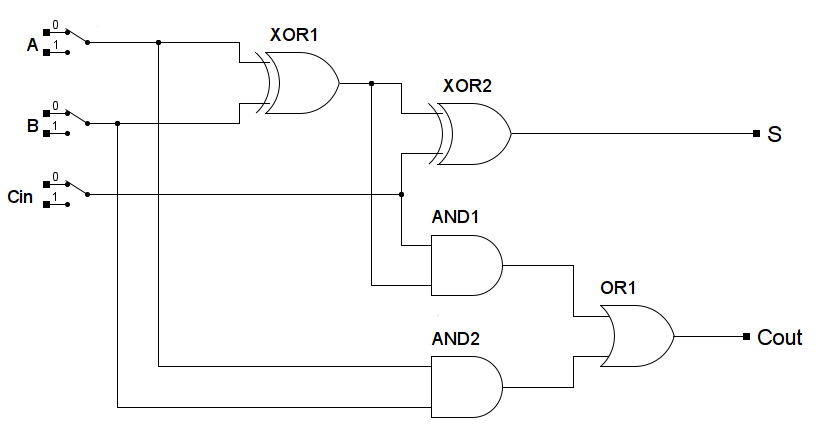
\includegraphics[scale=0.5]{\gitrepopath/examples/fulladder.png}
  \captionof{figure}{A circuit diagram of a full adder} \label{fig:fulladder}
  %\end{figure}
\end{center}

\begin{center}
  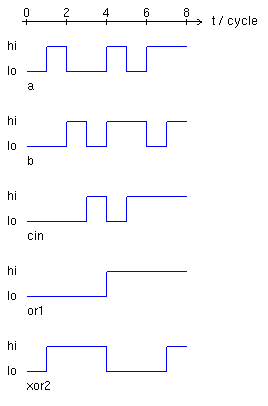
\includegraphics[scale=0.75]
                  {\gitrepopath/finalreport/fulladder_test.png}
  \captionof{figure}{Screenshot showing the successful test result
    of the full adder. Note that, compared to the definition
    file, additional monitors have been added.} \label{fig:testfulladder}
\end{center}

\subsection{Ripple counter}
\lstlistingname~\ref{lst:ripplecounter} and
\figurename~\ref{fig:ripplecounter} show a 4-bit ripple
counter, starts at 0, counts up to 15, and resets.
Note that this circuit has been modified to test the RC device
added during the maintenance stage, by forcing the devices to
start at 0. Its test result is reproduced in
\figurename~\ref{fig:testripplecounter}.

\lstinputlisting[caption={A 4-bit ripple counter described in the Logic
    Simulator format},label={lst:ripplecounter}]
                {\gitrepopath/examples/ripplecounter.circuit}
\begin{center}
  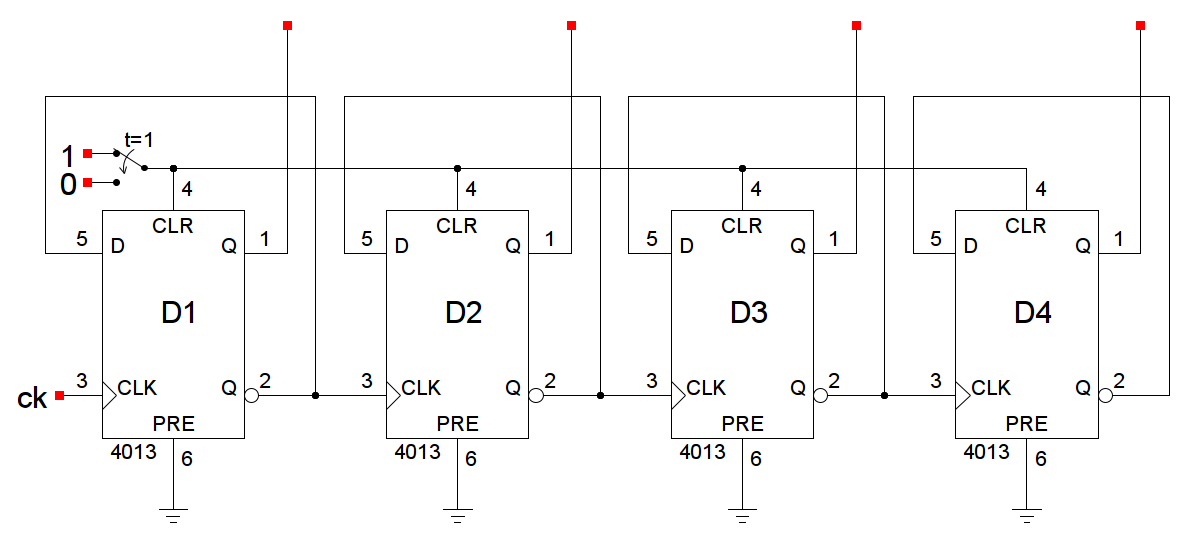
\includegraphics[width=\textwidth]{\gitrepopath/examples/ripplecounter.png}
  \captionof{figure}{A circuit diagram of a 4-bit ripple counter}
  \label{fig:ripplecounter}
\end{center}

\begin{center}
  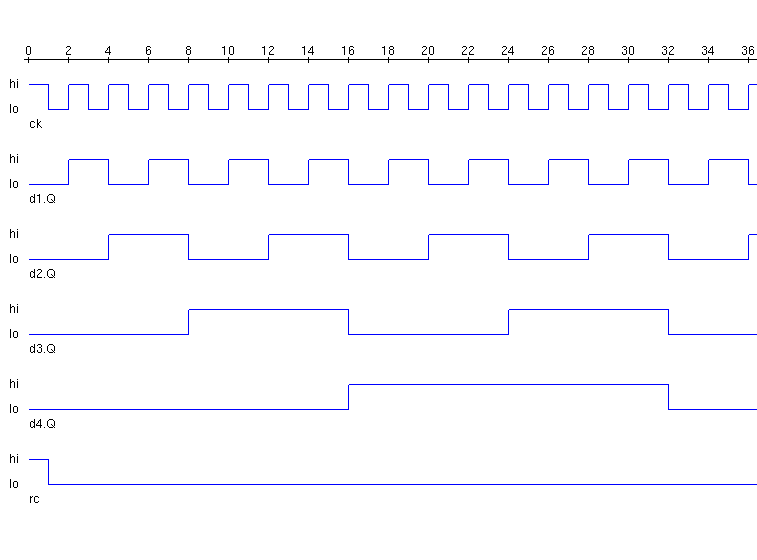
\includegraphics[width=\textwidth]
                  {\gitrepopath/finalreport/ripplecounter_test.png}
  \captionof{figure}{Screenshot showing the successful test result
    of the ripple counter. Note again that additional monitors
    have been added.} \label{fig:testripplecounter}
\end{center}

\subsection{8-to-1 multiplexer}
\lstlistingname~\ref{lst:8to1mux} and \figurename~\ref{fig:8to1mux}
show an 8-to-1 multiplexer
implemented using logic gates. In the \lstlistingname{}, the
three select lines are clocked such that the output will cycle from
\texttt{i0} to \texttt{i7} in an arbitrary order\footnote{Due to the
clocks not in sync.} and restart.
Note that the inverters
on the select lines are implemented both as the 1-input NAND gate
and also as the NOT gate added in the maintenance stage.

A test result is show in \figurename~\ref{fig:test8to1mux}.

\lstinputlisting[caption={An 8-to-1 multiplexer described in the Logic
    Simulator format},label={lst:8to1mux}]
                {\gitrepopath/examples/8to1mux.circuit}
\begin{center}
  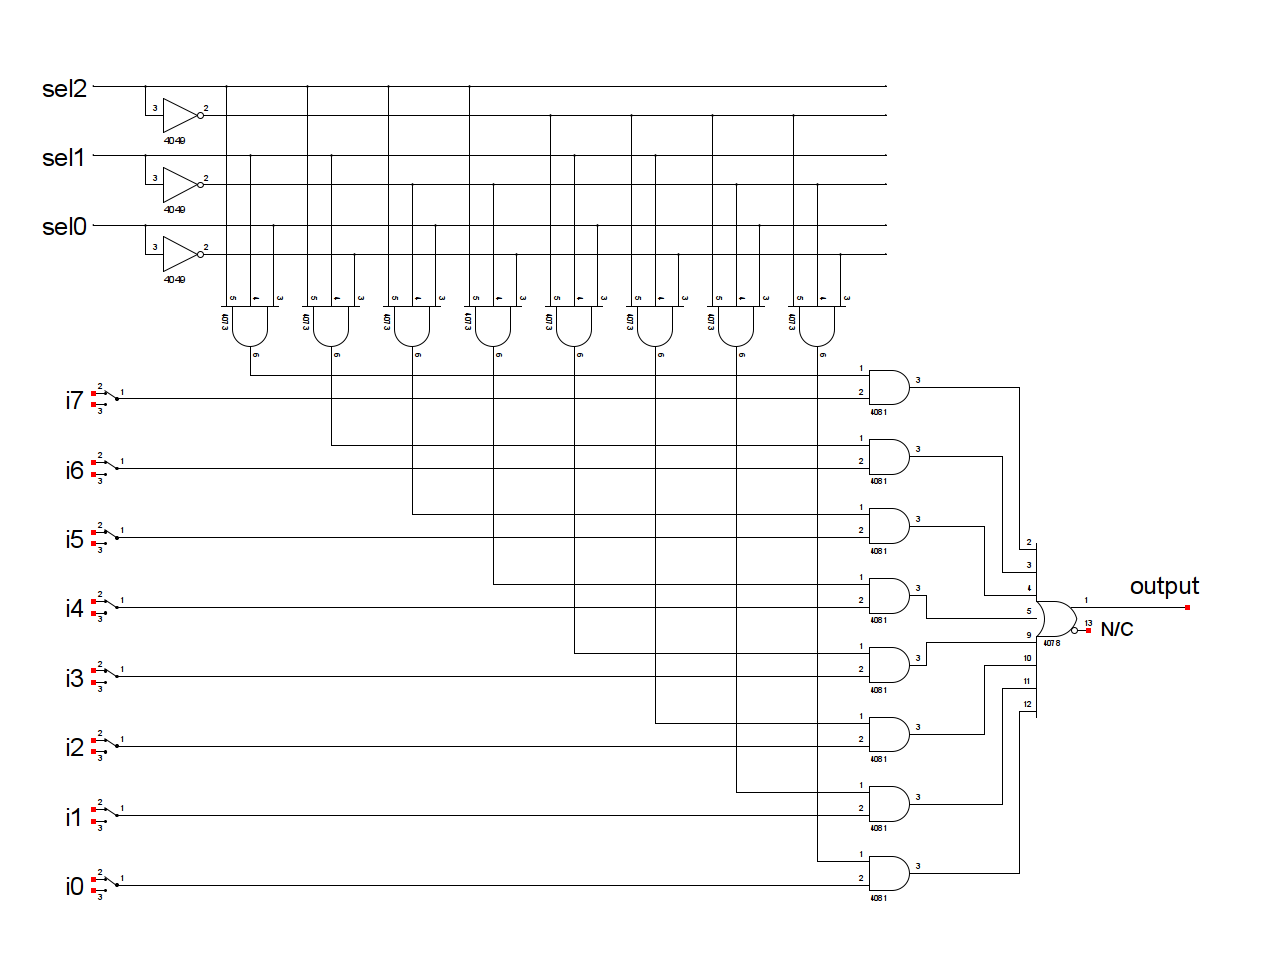
\includegraphics[width=\textwidth]{\gitrepopath/examples/8to1mux.png}
  \captionof{figure}{A circuit diagram of an 8-to-1 multiplexer}
  \label{fig:8to1mux}
\end{center}

\begin{center}
  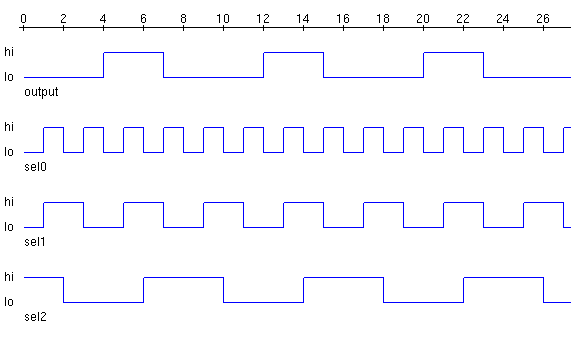
\includegraphics[width=\textwidth]
                  {\gitrepopath/finalreport/8to1mux_test.png}
   \captionof{figure}{Screenshot showing the successful test result
     of the 8-to-1 multiplexer, with inputs \texttt{i0}, \texttt{i3}, and
     \texttt{i6} set to 1, and other inputs set to 0.}
   \label{fig:test8to1mux}
\end{center}

\subsection{Sequence detector}
\lstlistingname~\ref{lst:1001seqdetect} and
\figurename~\ref{fig:1001seqdetect} show a sequence
detector for the input data sequence 1001. The data bit period should
be equal to 2. A high output at \texttt{and5} indicates a detected
sequence. \figurename~\ref{fig:test1001seqdetect} shows the test
result.

\lstinputlisting[caption={A sequence detector for sequence 1001
    described in the Logic Simulator format},label={lst:1001seqdetect}]
                {\gitrepopath/examples/1001seqdetect.circuit}
\begin{center}
  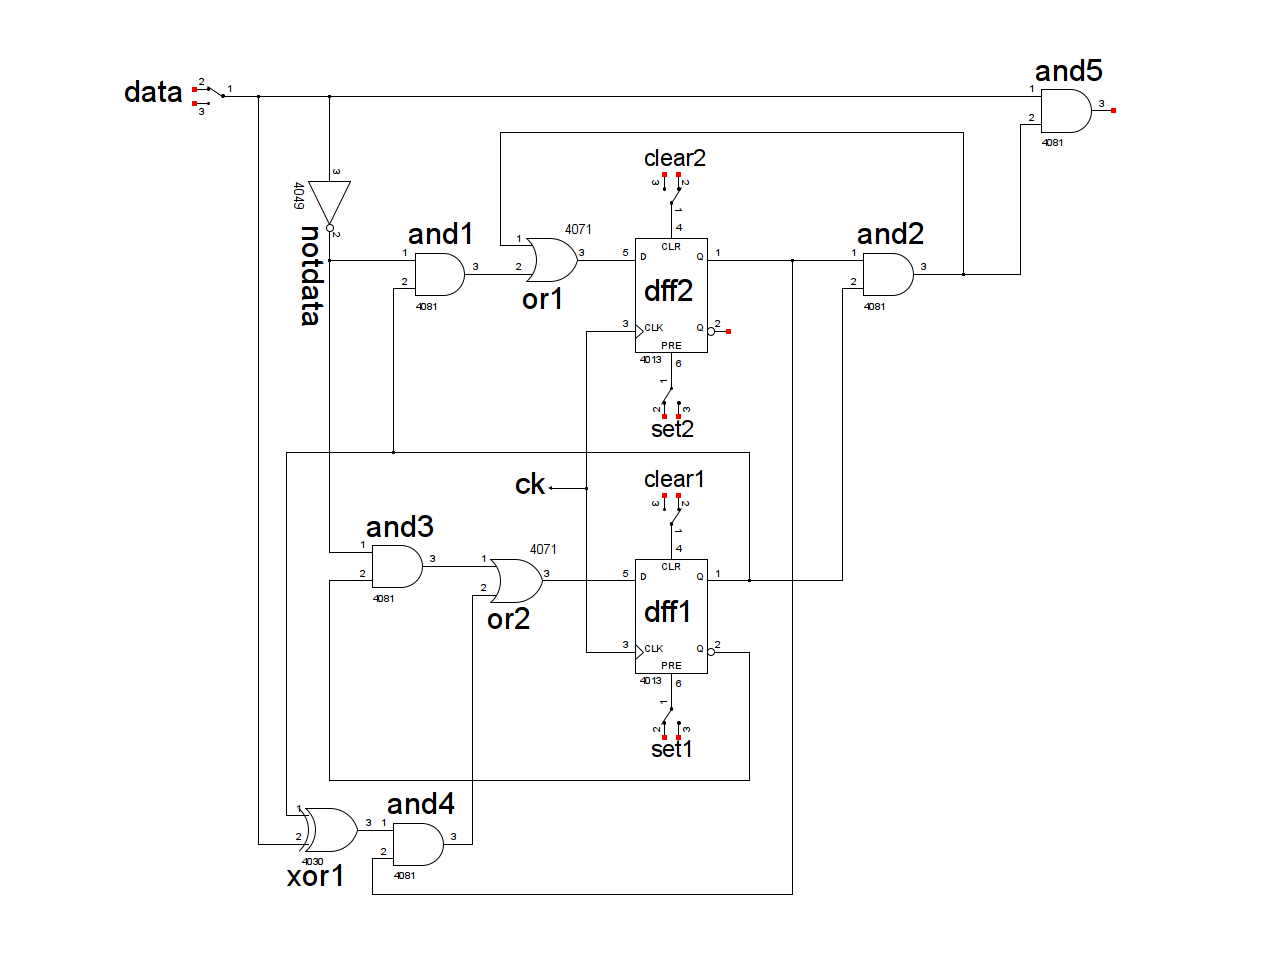
\includegraphics[width=\textwidth]{\gitrepopath/examples/1001seqdetect.png}
  \captionof{figure}{A circuit diagram of a sequence detector for
    sequence 1001}\label{fig:1001seqdetect}
\end{center}

\begin{center}
  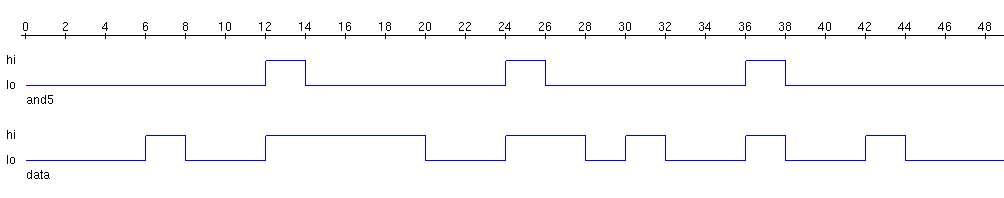
\includegraphics[width=\textwidth]
                  {\gitrepopath/finalreport/1001seqdetect_test.png}
  \captionof{figure}{Screenshot showing the successful test result
    of the sequence detector.} \label{fig:test1001seqdetect}
\end{center}
